\setlength\abovedisplayshortskip{15pt}
\setlength\belowdisplayshortskip{15pt}
\setlength\abovedisplayskip{15pt}
\setlength\belowdisplayskip{15pt}

\section{Theoretische Grundlagen \cite{Wedler}}




\begin{figure}[H]


     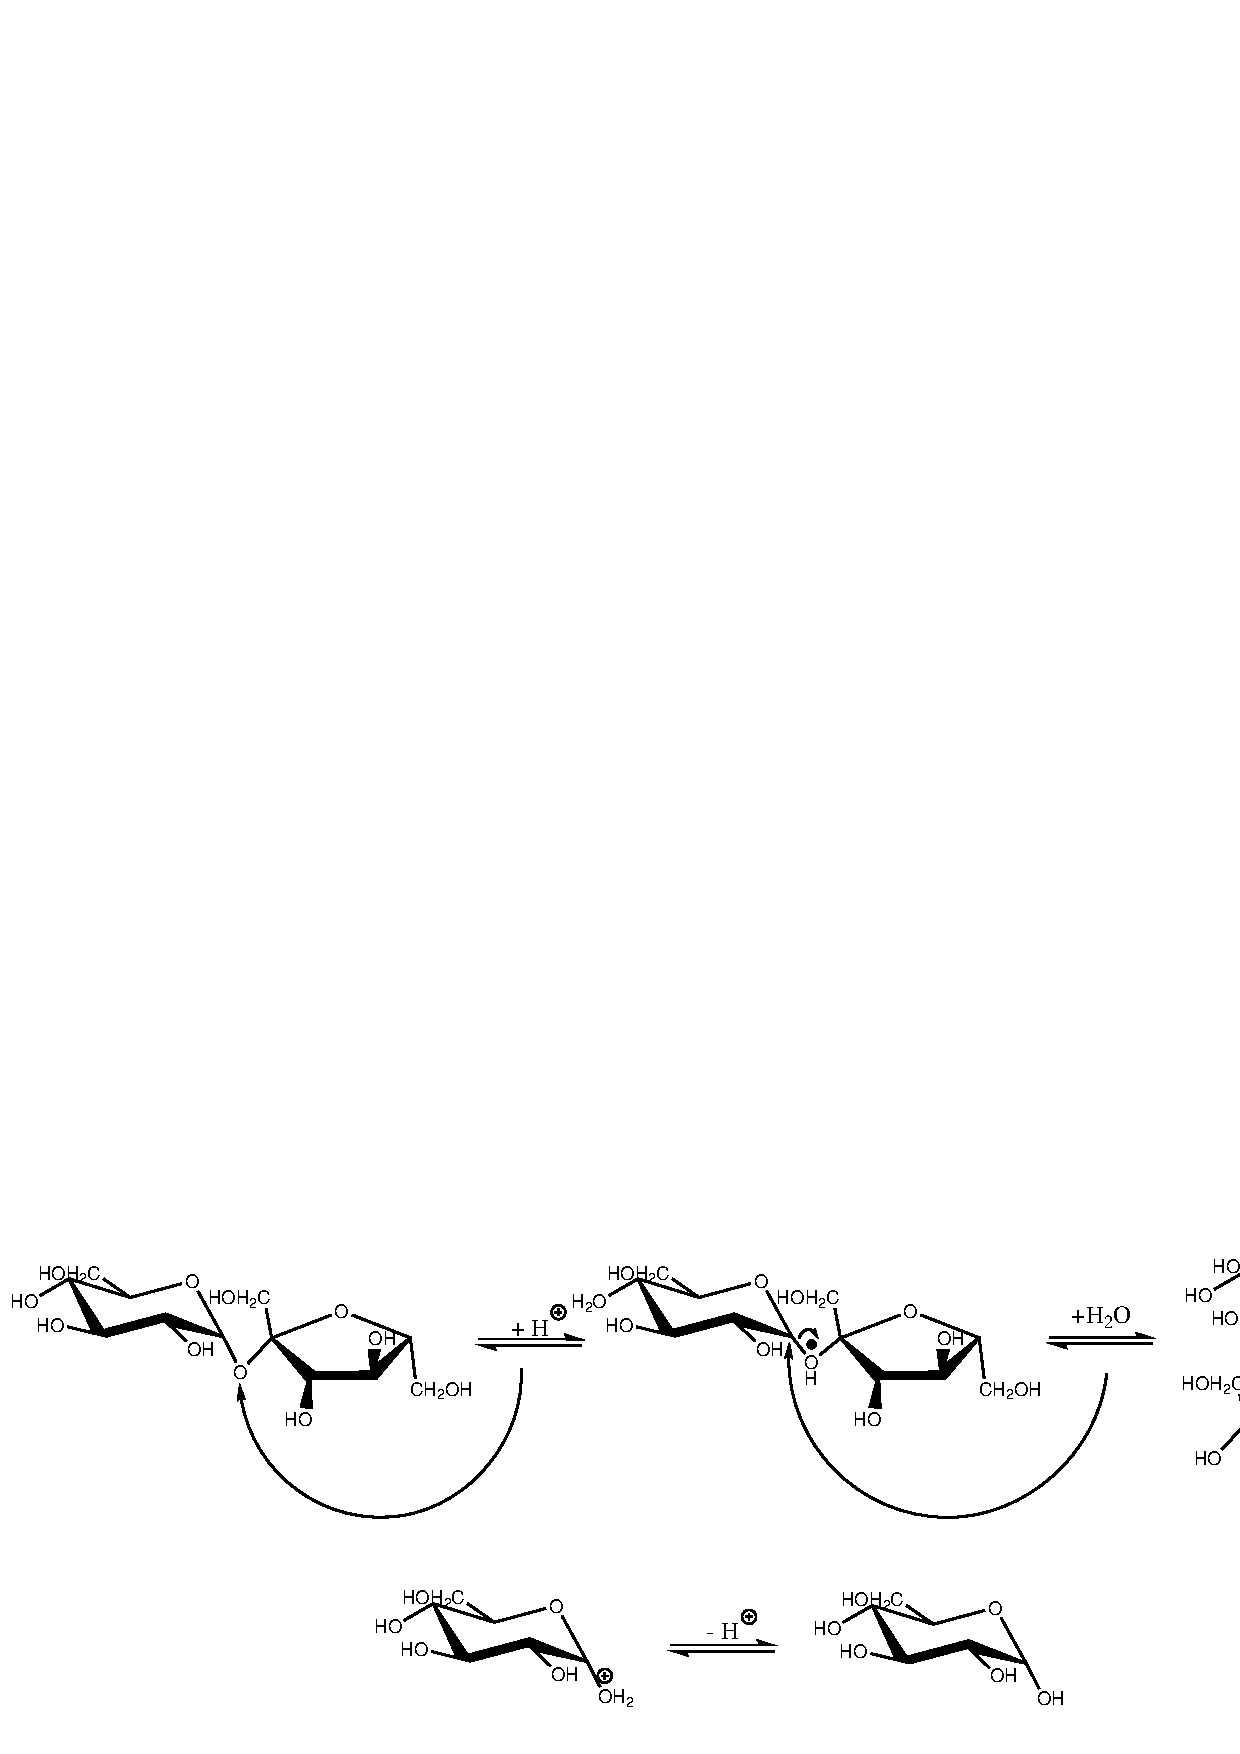
\includegraphics[width=1\linewidth]{Bilder/hydrolyse.png}
\caption{Mechanismus der säurekatalysierten Hydrolyse
von Saccharose in wässriger Lösung. Der einleitende Schritt ist
die Aktivierung des Sauerstoffatoms der Esterbindung durch Protonierung. Es folgt der nucleophile Angriff des Wassermoleküls und anschließende Hydrolyse des 
Disaccharids.}
\label{fig:hydrolyse}
\end{figure}

Die Reaktionsgleichung der Hydrolyse (vgl. Abbildung \ref{fig:hydrolyse}) von Saccharose [S] zu Fructose [F] und Glucose [G] lautet wie folgt: 

\begin{equation}
\ch{ \text{[S]} + [H]+ + H2O <=>[ $k_1$ ][ $k_{-1}$ ] \text{[S}H\text{]}+ + H2O ->[ $k_2$ ] \text{[F]} + \text{[G]} + [H]+  }
\label{Hydrolysegleichung}
\end{equation}
Die Reaktion verläuft unter Einsatz von katalytischen Mengen an Salzsäure und in wässriger Lösung, so dass die Hydrolyse irreversibel ist. Der geschwindigkeitsbestimmende Schritt der Reaktion ist der zweite Teil der Reaktion
\begin{align}
v = - \frac{d \text{[S]}}{dt}= k_2 \cdot \ch{\text{[S}H\text{]}+} \cdot \ch{[H2O]}
\label{eq:irreversibler2.Schritt}
\end{align}
wobei unter Verwendung des Quasistationaritätsprinzips gilt:
\begin{align}
\ch{\text{[S}H\text{]}+}=\frac{k_1}{\left(k_{-1} + k_2\right)}
 \cdot \ch{\text{[}H\text{]}+} \cdot \text{[S]}
 \label{eq:quasistationfürSH+}
\end{align}
,sodass nun ein Geschwindigkeitsgesetz 3. Ordnung aufgeschrieben werden kann.
\begin{align}
v = - \frac{d \text{[S]}}{dt}= K \cdot \ch{\text{[}H\text{]}+} \cdot \text{[S]} \cdot \ch{[H2O]}
\quad\quad \text{mit}\quad\quad  K=\frac{k_1}{\left(k_{-1} + k_2\right)}
 \cdot k_2
 \label{eq:Gesetz3.Ordnung}
\end{align}

Es wird nun jedoch zum einem angenommen, dass die Konzentration des Wasser konstant ist, da die Reaktion im wässrigen Medium durchgeführt wird und daher diese sich im Verlauf der Reaktion kaum ändert, zum anderen wird angenommen, dass die Konzentration der Protonen konstant ist, da es sich um einen katalytischen Prozess handelt. Das Geschwindigkeitsgesetzt ändert sich nun zu
\begin{equation}
v = - \frac{d \text{[S]}}{dt}= k \cdot \text{[S]}
\quad\quad \text{mit}\quad\quad  k=K\cdot\ch{\text{[}H\text{]}+} \cdot \ch{[H2O]}
\label{Pseudo1.Ordnung}
\end{equation}
Die Reaktion beschreibt also eine Geschwindigkeitsgesetz nach  1. Ordnung. Es wird auch in diesem Falle von einer Pseudo-Reaktion 1. Ordnung gesprochen. 



Die Anwendung der Operatoren liefert dann das integrierte Geschwindigkeitsgesetz:

\begin{equation}
\ch{[S]} = \ch{[S]0}\cdot e^{-kt}
\label{eq:integriertesGesetz}
\end{equation}

Um die Temperaturabhängigkeit der Reaktion zu ermitteln, nutzt man die Arrhenius-Gleichung:

\begin{equation}
k=k_\infty \cdot e^{ - \frac{E_A}{R \cdot T}}
\label{eq:Arrheniusgleichung}
\end{equation}

Dabei ist $k_\infty$ der sogenannte Frequenzfaktor, $E_A$ die Aktivierungsenergie, R die Gaskonstante und T die Temperatur.

Die graphische Auftragung ("Arrhenius-Plot") gelingt durch logarithmieren der oberen Gleichung:

\begin{equation}
ln(k)=ln(k_\infty)-\left( \frac{E_A}{ \text{R} \cdot T} \right)
\label{eq:logarithmArrhenius}
\end{equation}


Der Drehwinkel, der mit Hilfe eines Polarimeters gemessen werden kann, ist durch folgende Gleichung mit dem spezifischen Drehwinkel eines optisch aktiven Stoffes verknüpft:

\begin{equation}
\alpha=\left[\alpha\right]_\lambda^T \cdot l \cdot c
\label{eq:Drehwinkelallgemein}
\end{equation}

Dabei ist $l$ die Länge des Probenröhrchens , c die Konzentration der Probe und $\lambda$ die Wellenlänge des Lichtes (für gewöhnlich: $\lambda_\text{D}=589~\si{nm}$).

Dabei gilt, dass der zu messende Drehwinkel als Summe aus dem Produkten der molaren Drehwinkel $\alpha_{Zucker}^m  $ und derer in Lösung vorliegenden Zucker-Konzentrationen dargestellt werden kann.
\begin{equation}
\alpha=\alpha_S^m \cdot\text{[S]}+ \alpha_F^m \cdot\text{[F]}+ \alpha_G^m\cdot\text{[G]}
\end{equation}

Wobei vereinfacht werden kann da gilt $\text{[F]}=\text{[G]}$
\begin{equation}
\alpha=\alpha_S^m \cdot\text{[S]}+ \alpha_I^m \cdot\text{[I]} \quad\quad\quad \text{mit}\quad\quad\quad\alpha_I^m \cdot\text{[I]}=\alpha_F^m \cdot\text{[F]}+ \alpha_G^m\cdot\text{[G]}\
\end{equation}

Und da ebenso gilt bei $t=0$ ist $\text{[I]}= 0$ und $\text{[S]}=\text{[S]}_0-\text{[I]}$ kann geschrieben werden
\begin{equation}
\alpha=\alpha_S^m \cdot(\text{[S]}_0-\text{[I]})+  \alpha_I^m \cdot\text{[I]}
\end{equation}
beziehungsweise
\begin{equation}
\text{[I]} =\frac{\alpha_S^m \cdot\text{[S]}_0 - \alpha }{\alpha_I^m-\alpha_S^m} 
\label{gleichung 13}
\end{equation}
Wobei des weiteren zwei Grenzfälle unterschieden werden können
\begin{equation} 
   \begin{cases}
      \alpha_0 =\alpha_S^m \cdot\text{[S]}_0 & \text{f"ur } t=0\\
       \alpha_{\infty} =\alpha_I^m \cdot\text{[S]}_0 & \text{f"ur } t=\infty\\
     \end{cases}
\end{equation}
sodass Gleichung \ref{gleichung 13} zu 
\begin{equation}
\text{[I]} =\frac{\alpha_0 - \alpha }{\alpha_{\infty}-\alpha_0} \cdot \text{[S]}_0
\end{equation}
vereinfacht werden kann.

Dies eingesetzt in Gleichung \ref{eq:integriertesGesetz} immer noch unter Annahme von $\text{[S]}=\text{[S]}_0-\text{[I]}$ führt zu folgenden Ausdruck


\begin{align}
\ch{[S]}_0-\frac{\alpha_0 - \alpha }{\alpha_{\infty}-\alpha_0} \cdot \text{[S]}_0 &= \ch{[S]0}\cdot e^{-kt} \\[10pt]
1-\frac{\alpha_0 - \alpha }{\alpha_{\infty}-\alpha_0} &= e^{-kt}
\end{align}

Der Drehwinkel lässt sich also als eine sich linear mit dem Verlauf der Reaktion verändernde Funktion der Zeit begreifen.

\begin{equation}
\alpha(t)= (\alpha_0 - \alpha_\infty) \cdot e^{(-kt)}+\alpha_{\infty}
\label{eq:winkelvontfunktion}
\end{equation}

$\alpha_0$ = Drehwinkel zu Beginn der Reaktion, $\alpha_\infty$ = Drehwinkel am Ende der Reaktion.



